\documentclass[dvipdfm,serif,mathserif]{beamer}
\usepackage{color}
\usepackage{amsmath, amsfonts, epsfig, xspace}
\usepackage{algorithm,algorithmic}
\usepackage{pstricks,pst-node}
\usepackage{multimedia}
\usepackage[normal,tight,center]{subfigure}
\usepackage[boldfont,slantfont,CJKnumber]{xeCJK}
\usepackage{graphicx}
\usepackage{booktabs}
\usepackage{longtable}
\usepackage{array}
\usepackage{multicol}
\usepackage{colortbl}

\setCJKmainfont[BoldFont=Adobe Heiti Std]{Adobe Song Std} % 设置默认的中文字体
\setCJKfamilyfont{kai}{Adobe Kaiti Std}

\definecolor{darkgreen}{rgb}{0,.39,0}

\renewcommand{\textdollar}{{\char"0024}}
\renewcommand{\today}{\number\year 年 \number\month 月 \number\day 日}
\usetheme{Montpellier}

\definecolor{steelblue}{rgb}{.275,.51,.71}
\definecolor{lpink}{rgb}{.991,.711,.754}
\definecolor{mygray}{gray}{0.92}
\definecolor{darkblue}{rgb}{0,0,.5}
\definecolor{darkgreen}{rgb}{0,.39,0}
\definecolor{hgray}{gray}{.5}
\definecolor{lgray}{gray}{.8}
\definecolor{mypink}{rgb}{.99,.91,.95}

\graphicspath{{data/}} %%图片路径
%  \DeclareGraphicsExtensions{.}
  \hypersetup{pdfpagemode={FullScreen}} % 全屏幕

\begin{document}

% \author{颜开}
\title{   \textcolor{darkgreen}{\textbf{iMath}}}
\date{\today}
\author{Jerry Mouse}

\begin{frame}
\framesubtitle{}
  \titlepage
\end{frame}

\begin{frame}\frametitle{目录}
\tableofcontents

\end{frame}


\AtBeginSection[] {
  \frame<handout:0> {
    \frametitle{目录}
    \tableofcontents[current]
  }
}

\section{胡吹大气iMath}

\subsection{网站地址}
\begin{frame}
  \frametitle{网站地址}
\begin{LARGE}\href{http://i-math.appspot.com/}{\color{blue}http://i-math.appspot.com/}
\end{LARGE}\end{frame}

\subsection{软件功能}
\begin{frame}
  \frametitle{横向软件对比}
\begin{center}

\begin{tabular}{m{0.4\textwidth}m{0.4\textwidth}}
\toprule
iMath & 传统数学软件 \\
\midrule
\rowcolor{lgray}
免费   & 昂贵 \\
轻型快速   & 趋于笨重   \\
\rowcolor{lgray}
灵活,个性化    & 单一普适   \\
\bottomrule
\end{tabular}

\end{center}
\end{frame}

\begin{frame}
  \frametitle{特点}
\begin{itemize}
\item 基本操作:拖拽,添加,删除 功能模块
\item 开放式添加 功能模块
\item AOP缓存系统
\item 测试系统:\href{http://i-math.appspot.com/ifr.action?url=http://i-math.appspot.com/gadgets/add-gadget/add-gadget.xml}{\color{blue}测试地址}
\item Gadget互操作实现
\item \href{http://i-math.appspot.com/dwr/index.html}{\color{blue}Rest Rpc式的webService实现}
\end{itemize}
\end{frame}


\subsection{项目规模}

\begin{frame}
  \frametitle{项目规模}
\begin{itemize}
\begin{minipage}[c]{0.6\textwidth}
\item 23个子项目
\item 26655 行各种代码
\item 1641 行构建代码
  \end{minipage}
  \begin{minipage}[c]{0.3\textwidth}
  \includegraphics[width=\textwidth]{eclipse.ps}
  \end{minipage}
\end{itemize}
\end{frame}

\begin{frame}
  \frametitle{项目结构}
\begin{itemize}
 \item i-math-web
\item gadgets
\begin{itemize}
 \item cache
 \item calculator
 \item latex2image
 \item smartcalculator
 \item ...
\end{itemize}
\end{itemize}
\end{frame}

\section{开发所得}
\subsection{让应用部署在公网上}

\begin{frame}
  \frametitle{It's impossible}
\begin{itemize}
\begin{minipage}[c]{0.6\textwidth}
 \item 使用自己的电脑+动态域名
 \item 使用免费托管服务
\item 那就用付费的吧
\item 去机房租台
\item 挪用软院的服务器
\pause
 \item \href{http://code.google.com/appengine/}{\color{blue}Google App Engine}
  \end{minipage}
  \begin{minipage}[c]{0.3\textwidth}
  
\includegraphics[width=\textwidth]{appengine_lowres.ps}
  \end{minipage}
\end{itemize}
\end{frame}

\begin{frame}
  \frametitle{哪些挑战}
\begin{itemize}
\item 一个有洁癖的服务器沙箱
\begin{itemize}
 \item Spring,Struts,CXF.....
\end{itemize}
\item 没有完全实现的Java类库
\begin{itemize}
 \item javax.ws,osgi.....
\end{itemize}
\item BigTable
\item 集群服务器
\item 速度非快
\end{itemize}
\end{frame}

\begin{frame}
  \frametitle{BigTable with his bugs}
\framesubtitle{BigTable  是构建在Goolge文件系统 (GFS) 上的高性能 压缩的 列数据库.}
\begin{itemize}
\item JDO \& JPA 接口
\item 列数据库
\begin{itemize}
 \item 你得自己构建索引
\end{itemize}
 \item \href{http://appengine.google.com/}{\color{blue}管理界面}
\end{itemize}
\end{frame}

\subsection{RIA有感}

\begin{frame}
  \frametitle{RIA有感}
\begin{itemize}
\item Flex
\item SliverLight
\item Curl
\item Html5+Javascript
\end{itemize}
\end{frame}

\begin{frame}
  \frametitle{JavaScript框架}
\begin{itemize}
\item Dojo:妄图包揽一切的集大成者
\item JQuery:开放的社区,霸道的设计
\item Ext+Gwt:无敌组合
\item Mootools:简单就是美
\end{itemize}
\end{frame}

\section{Q \& A}
\begin{frame}
\begin{Huge}\begin{center}
            \textbf{  Q \& A}
             \end{center}\end{Huge}
\end{frame}
\end{document}
